\documentclass{beamer}

\usepackage{tikz}
\usepackage{pdfpages}

% switch off the fancy navigation symbols
\setbeamertemplate{navigation symbols}{}

\title{${}$\\[3.5em]11th International\\
Satisfiability Modulo Theories\\
Competition\\[.7em]
SMT-COMP 2016\\[3em]}

\author{Sylvain Conchon \and David D{\'e}harbe \and Matthias Heizmann \and Tjark Weber}

\institute{}

\date{}

\logo{\vspace{2.7cm}\includegraphics[width=\textwidth]{laurels}\hspace{.8cm}}

\begin{document}

%%%%%%%%%%%%%%%%%%%%%%%%%%%%%%%%%%%%%%%%%%%%%%%%%%%%%%%%%%%%%%%%%%%%%%%%%%%%%%%%

\frame{\titlepage}
\logo{}

%%%%%%%%%%%%%%%%%%%%%%%%%%%%%%%%%%%%%%%%%%%%%%%%%%%%%%%%%%%%%%%%%%%%%%%%%%%%%%%%

\section{}% leave this empty
\subsection{}% leave this empty

%%%%%%%%%%%%%%%%%%%%%%%%%%%%%%%%%%%%%%%%%%%%%%%%%%%%%%%%%%%%%%%%%%%%%%%%%%%%%%%%

\begin{frame}{The Numbers}
  \begin{itemize}
  \item 17 teams participated
    \smallskip
  \item Solvers:\\
    \smallskip
    \usebeamercolor{structure}
    \begin{tikzpicture}
      \draw (0,-.25) -- (0,1.25);
      \node [left] at (0,1) {\footnotesize Main track};
      \node [left] at (0,.5) {\footnotesize Application track};
      \node [left] at (0,0) {\footnotesize Unsat-core track};

      \draw [fill=fg] (0,.85) rectangle (3.571428571,1.15);
      \node [left,white] at (3.571428571,1) {\footnotesize 25};
      \draw [fill=fg!30!white] (3.571428571,.85) rectangle (3.857142857,1.15);
      \node [right] at (3.857142857,1) {\tiny 2 non-competitive};

      \draw [fill=fg] (0,.35) rectangle (1.142857143,.65);
      \node [left,white] at (1.142857143,.5) {\footnotesize 8};
      \draw [fill=fg!30!white] (1.142857143,.35) rectangle (1.571428571,.65);
      \node [right] at (1.571428571,.5) {\tiny 3 non-competitive};

      \draw [fill=fg] (0,-.15) rectangle (.142857143,.15);
      \draw [fill=fg!30!white] (.142857143,-.15) rectangle (.714285714,.15);
      \node [right,black] at (.142857143,0) {\footnotesize 1};
      \node [right] at (.714285714,0) {\tiny 4 non-competitive};
    \end{tikzpicture}
  \item Logics:\\
    \smallskip
    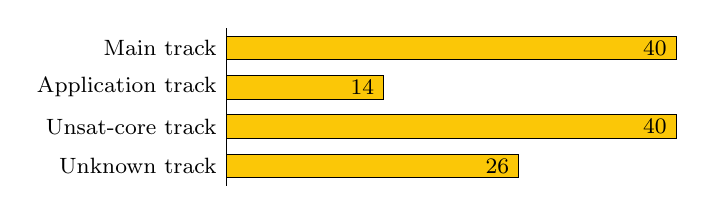
\begin{tikzpicture}
      \draw (0,-.75) -- (0,1.25);
      \node [left] at (0,1) {\footnotesize Main track};
      \node [left] at (0,.5) {\footnotesize Application track};
      \node [left] at (0,0) {\footnotesize Unsat-core track};
      \node [left] at (0,-.5) {\footnotesize Unknown track};

      \draw [fill=yellow!80!red] (0,.85) rectangle (5.714285714,1.15);
      \node [left] at (5.714285714,1) {\footnotesize 40};

      \draw [fill=yellow!80!red] (0,.35) rectangle (2,.65);
      \node [left] at (2,.5) {\footnotesize 14};

      \draw [fill=yellow!80!red] (0,-.15) rectangle (5.714285714,.15);
      \node [left] at (5.714285714,0) {\footnotesize 40};

      \draw [fill=yellow!80!red] (0,-.65) rectangle (3.714285714,-.35);
      \node [left] at (3.714285714,-.5) {\footnotesize 26};
    \end{tikzpicture}
  \item Benchmarks:\\
    \smallskip
    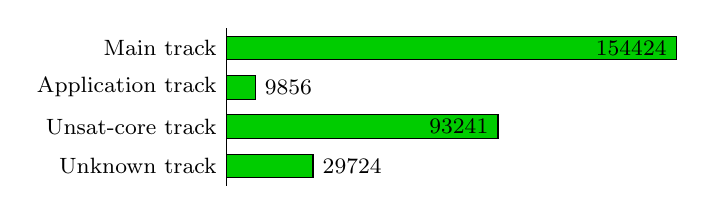
\begin{tikzpicture}
      \draw (0,-.75) -- (0,1.25);
      \node [left] at (0,1) {\footnotesize Main track};
      \node [left] at (0,.5) {\footnotesize Application track};
      \node [left] at (0,0) {\footnotesize Unsat-core track};
      \node [left] at (0,-.5) {\footnotesize Unknown track};

      \draw [fill=green!80!black] (0,.85) rectangle (5.714285714,1.15);
      \node [left] at (5.714285714,1) {\footnotesize 154424};

      \draw [fill=green!80!black] (0,.35) rectangle (0.365001769,.65);
      \node [right] at (0.365001769,.5) {\footnotesize 9856};

      \draw [fill=green!80!black] (0,-.15) rectangle (3.450277899,.15);
      \node [left] at (3.450277899,0) {\footnotesize 93241};
      
      \draw [fill=green!80!black] (0,-.65) rectangle (1.09990305,-.35);
      \node [right] at (1.09990305,-.5) {\footnotesize 29724};
    \end{tikzpicture}
  \end{itemize}

  \vspace{-\smallskipamount}
  
  \structure{Record numbers} of solvers and benchmarks!
\end{frame}

%%%%%%%%%%%%%%%%%%%%%%%%%%%%%%%%%%%%%%%%%%%%%%%%%%%%%%%%%%%%%%%%%%%%%%%%%%%%%%%%

\begin{frame}{Job Pairs}
  \begin{itemize}
  \item \structure{1,562,544} job pairs executed (+ some repeats)
  \end{itemize}

  \begin{center}
    \usebeamercolor{structure}
    \begin{tikzpicture}
      \draw [gray] (0,0) -- (10,0);
      \draw [gray] (0,.9) -- (10,.9);
      \draw [gray] (0,1.8) -- (10,1.8);
      \draw [gray] (0,2.7) -- (10,2.7);
      \draw [gray] (0,3.6) -- (10,3.6);
      \draw [gray] (0,4.5) -- (10,4.5);

      \node [left,gray] at (0,0) {\tiny 0};
      \node [left,gray] at (0,.9) {\tiny 300,000};
      \node [left,gray] at (0,1.8) {\tiny 600,000};
      \node [left,gray] at (0,2.7) {\tiny 900,000};
      \node [left,gray] at (0,3.6) {\tiny 1,200,000};
      \node [left,gray] at (0,4.5) {\tiny 1,500,000};

      \draw [fill=fg!30!white] (1,0) rectangle (3,1.019142);
      \draw [fill=fg!30!white] (4,0) rectangle (6,3.085845);
      \draw [fill=fg] (7,0) rectangle (9,4.687632);

      \node [below,gray] at (2,0) {\footnotesize SMT-COMP 2014};
      \node [below,gray] at (5,0) {\footnotesize SMT-COMP 2015};
      \node [below] at (8,0) {\footnotesize SMT-COMP 2016};
    \end{tikzpicture}
  \end{center}
\end{frame}

%%%%%%%%%%%%%%%%%%%%%%%%%%%%%%%%%%%%%%%%%%%%%%%%%%%%%%%%%%%%%%%%%%%%%%%%%%%%%%%%

\begin{frame}{Job Pairs by Track}
\def\angle{0}
\def\radius{3}
\def\cyclelist{{"blue","green","red","yellow"}}
\newcount\cyclecount \cyclecount=-1
\newcount\ind \ind=-1
\begin{center}
\begin{tikzpicture}[nodes = {font=\sffamily}]
  \foreach \percent/\name in {
      64.2/Main track,
      22.0/Unknown track,
      11.7/Unsat-core track,
      2.1/Application track,
    } {
      \ifx\percent\empty\else               % If \percent is empty, do nothing
        \global\advance\cyclecount by 1     % Advance cyclecount
        \global\advance\ind by 1            % Advance list index
        \ifnum3<\cyclecount                 % If cyclecount is larger than list
          \global\cyclecount=0              %   reset cyclecount and
          \global\ind=0                     %   reset list index
        \fi
        \pgfmathparse{\cyclelist[\the\ind]} % Get color from cycle list
        \edef\color{\pgfmathresult}         %   and store as \color
        % Draw angle and set labels
        \draw[fill={\color!50},draw={\color}] (0,0) -- (\angle:\radius)
          arc (\angle:\angle+\percent*3.6:\radius) -- cycle;
        \node at (\angle+0.5*\percent*3.6:0.7*\radius) {\percent\,\%};
        \node[pin=\angle+0.5*\percent*3.6:\name]
          at (\angle+0.5*\percent*3.6:\radius) {};
        \pgfmathparse{\angle+\percent*3.6}  % Advance angle
        \xdef\angle{\pgfmathresult}         %   and store in \angle
      \fi
    };
\end{tikzpicture}
\end{center}
\end{frame}

%%%%%%%%%%%%%%%%%%%%%%%%%%%%%%%%%%%%%%%%%%%%%%%%%%%%%%%%%%%%%%%%%%%%%%%%%%%%%%%%

\begin{frame}{StarExec}
  \begin{itemize}
  \item All job pairs executed on StarExec
  \item Timeout: \structure{40 minutes} (unknown track: 10 minutes)
  \item $\sim$ \structure{12 days $\times$ 100 nodes $\times$ 2
    processors/node} of compute time
  \end{itemize}

  \medskip

  \begin{center}
    {\Large\structure{StarExec worked even better than last year}}
  \end{center}

  \medskip

  \begin{itemize}
  \item Thanks to Aaron Stump for prompt help when problems or
    questions arose
  \item Only very few (and minor) bug reports submitted to the
    StarExec developers
  \end{itemize}
\end{frame}

%%%%%%%%%%%%%%%%%%%%%%%%%%%%%%%%%%%%%%%%%%%%%%%%%%%%%%%%%%%%%%%%%%%%%%%%%%%%%%%%

\begin{frame}{Machine Specifications}
  Hardware:
  \begin{itemize}
  \item Intel Xeon CPU E5-2609 @ 2.4 GHz, 10 MB cache
  \item 2 processors per node, 4 cores per processor
  \item Main memory capped at 60~GB per job pair
  \end{itemize}

  \bigskip

  Software (\structure{upgraded in 2016}):
  \begin{itemize}
  \item Red Hat Enterprise Linux Server release 7.2
  \item Kernel 3.10.0-327, gcc 4.8.5, glibc 2.17
  \item Virtual machine image available before the competition
  \end{itemize}
\end{frame}

%%%%%%%%%%%%%%%%%%%%%%%%%%%%%%%%%%%%%%%%%%%%%%%%%%%%%%%%%%%%%%%%%%%%%%%%%%%%%%%%

\begin{frame}{Benchmarks and Logics}
  \begin{itemize}
  \item Number of benchmarks in SMT-LIB almost unchanged since 2015
    \smallskip
    \begin{itemize}
    \item Very few new benchmarks
    \item Some non-conforming benchmarks were removed
    \end{itemize}
    \medskip
  \item No new logics
    \medskip
  \item Thanks to Clark Barrett for curation and uploading
  \end{itemize}
\end{frame}

%%%%%%%%%%%%%%%%%%%%%%%%%%%%%%%%%%%%%%%%%%%%%%%%%%%%%%%%%%%%%%%%%%%%%%%%%%%%%%%%

\begin{frame}{Eligible Benchmarks}
  \begin{center}
    \usebeamercolor{structure}
    \begin{tikzpicture}[yscale=2]
      \draw [gray] (0,0) -- (3.75,0); \draw [gray] (4.25,0) -- (8,0);
      \draw [gray] (0,.5) -- (3.75,.5); \draw [gray] (4.25,.5) -- (8,.5);
      \draw [gray] (0,1) -- (3.75,1); \draw [gray] (4.25,1) -- (8,1);
      \draw [gray] (0,1.5) -- (3.75,1.5);
      \draw [gray] (0,2) -- (3.75,2);
      \node [left,gray] at (0,0) {\tiny 0};
      \node [left,gray] at (0,1) {\tiny 100,000};
      \node [left,gray] at (0,2) {\tiny 200,000};
      \node [right,gray] at (8,0) {\tiny 0};
      \node [right,gray] at (8,.5) {\tiny 5,000};
      \node [right,gray] at (8,1) {\tiny 10,000};
      \draw [fill=lightgray] (1,1.66204) rectangle (3,1.96375);
      \draw [fill=orange] (1,1.54238) rectangle (3,1.66204);
      \draw [fill=fg] (1,0) rectangle (3,1.54238);
      \draw [fill=lightgray] (5,0.9852) rectangle (7,1.0019);
      \draw [fill=fg] (5,0) rectangle (7,0.9852);
      \node at (2,1.812895) {\tiny status unknown};
      \node at (2,1.60221) {\tiny partial operations};
      \node [white] at (2,0.77119) {\tiny eligible};
      \node [above] at (6,0.99355) {\tiny status unknown};
      \node [white] at (6,0.4926) {\tiny eligible};
      \node [below] at (2,0) {\small Main track};
      \node [below] at (6,0) {\small Application track};
    \end{tikzpicture}
  \end{center}

  All eligible benchmarks were used for the competition.  There was
  \structure{no further selection}.
\end{frame}

%%%%%%%%%%%%%%%%%%%%%%%%%%%%%%%%%%%%%%%%%%%%%%%%%%%%%%%%%%%%%%%%%%%%%%%%%%%%%%%%

\begin{frame}{Important Rule Changes}
  \begin{itemize}
  \item \structure{SMT-LIB~2.5} instead of~2.0
    \begin{itemize}
    \item SMT-LIB not fully migrated yet
    \item Fortunately, largely backwards-compatible
    \end{itemize}
    \bigskip
  \item Size-based \structure{weighting of benchmark families} within
    divisions:
    $$1 + \log_e |F|$$
    Small benchmark families are more important than before.
    \bigskip
  \item \structure{Unsat-core track} reinstated
  \end{itemize}
\end{frame}

%%%%%%%%%%%%%%%%%%%%%%%%%%%%%%%%%%%%%%%%%%%%%%%%%%%%%%%%%%%%%%%%%%%%%%%%%%%%%%%%

% Source: http://www.clker.com/clipart-quality-control-approved-1.html
\logo{
\includegraphics[width=2.5cm]{quality-control-approved}}

\begin{frame}{Competition Tools Improved}
  \begin{itemize}
  \item New \structure{unsat-core track tools} (scrambler and
    post-processor)

    \bigskip

  \item New \structure{scrambling algorithm} that makes it harder to
    identify the original benchmark (cf.\ yesterday's talk)
  \end{itemize}
  \bigskip
\end{frame}

\logo{}

%%%%%%%%%%%%%%%%%%%%%%%%%%%%%%%%%%%%%%%%%%%%%%%%%%%%%%%%%%%%%%%%%%%%%%%%%%%%%%%%

\begin{frame}{}
  \begin{center}
    \vfill
      {\huge \structure{Solvers}}
    \vfill
  \end{center}
\end{frame}

{
  \setbeamercolor{background canvas}{bg=}
  \includepdf{AProVE.pdf}
  \includepdf{OpenSMT2.pdf}
  \includepdf{raSAT.pdf}
  \includepdf{veriT.pdf}
}

%%%%%%%%%%%%%%%%%%%%%%%%%%%%%%%%%%%%%%%%%%%%%%%%%%%%%%%%%%%%%%%%%%%%%%%%%%%%%%%%

\begin{frame}{}
  \begin{center}
    \vfill
      {\huge \structure{Selected Results}}
    \vfill
  \end{center}
\end{frame}

%%%%%%%%%%%%%%%%%%%%%%%%%%%%%%%%%%%%%%%%%%%%%%%%%%%%%%%%%%%%%%%%%%%%%%%%%%%%%%%%

\begin{frame}{Results: QF\_BV (Main Track)}
  \begin{tabular}{lrrr}
Solver          & Error Score & Solved Score (Parallel) & Unsolved \\ \hline
{\bf Boolector (pre)} & {\bf 0.000} & {\bf 24473.995} & {\bf 149} \\
Boolector 	& 0.000	& 24468.395 & 150 \\
Minkeyrink 	& 0.000	& 24434.194 & 193 \\
smt-cms-mt 	& 0.000	& 24244.599 & 216 \\
smt-cms-st 	& 0.000	& 24165.007 & 214 \\
CVC4 	        & 0.000	& 23820.707 & 231 \\
\textcolor{gray}{Z3} & \textcolor{gray}{0.000} & \textcolor{gray}{23732.215} & \textcolor{gray}{304} \\
smt-cms-exp 	& 0.000	& 23640.669 & 270 \\
ABC\_glucose 	& 0.000	& 23078.931 & 477 \\
Yices2 	        & 0.000	& 22687.777 & 638 \\
\textcolor{gray}{MathSat5} & \textcolor{gray}{0.000} & \textcolor{gray}{22496.779} & \textcolor{gray}{544} \\
MapleSTP-mt 	& 0.000	& 22487.264 & 395 \\
MapleSTP 	& 0.000	& 21764.885 & 450 \\
smt-minisat-st 	& 0.000	& 20582.614 & 1058 \\
ABC\_default 	& 0.000	& 18528.788 & 1354 \\
Q3B 	        & 719.723 & 10397.757 & 4430
  \end{tabular}  
\end{frame}

%%%%%%%%%%%%%%%%%%%%%%%%%%%%%%%%%%%%%%%%%%%%%%%%%%%%%%%%%%%%%%%%%%%%%%%%%%%%%%%%

\begin{frame}{Results: Competition-Wide Scoring (Main Track)}
  \begin{tabular}{llrr}
    Rank & Solver & Score (sequential) & Score (parallel)\\ \hline
         & \textcolor{gray}{Z3} & \textcolor{gray}{185.09} & \textcolor{gray}{185.09} \\
    1    & CVC4   & 180.95             & 181.19 \\
    2    & Yices  & 119.29             & 119.29 \\
    3    & veriT  & 75.11              & 75.11 \\
    \\
    \\
    \multicolumn{3}{l}{Best newcomer:}\\
    \\
    5    & Vampire\_parallel & 65.36 & 65.62	
  \end{tabular}  
\end{frame}

%%%%%%%%%%%%%%%%%%%%%%%%%%%%%%%%%%%%%%%%%%%%%%%%%%%%%%%%%%%%%%%%%%%%%%%%%%%%%%%%

\begin{frame}{Results: Application Track (Summary)}
  \begin{tabular}{ll}
    Logic       & Order \\ \hline
    ANIA	& \textcolor{gray}{Z3; CVC4} \\
    QF\_ANIA	& \textcolor{gray}{Z3; CVC4} \\
    QF\_ALIA	& \textcolor{gray}{Z3;} SMTInterpol; Yices2; \textcolor{gray}{MathSat5; CVC4} \\
    QF\_UFNIA	& \textcolor{gray}{Z3; CVC4} \\
    LIA         & \textcolor{gray}{Z3; CVC4} \\
    ALIA	& \textcolor{gray}{Z3; CVC4} \\
    QF\_UFLRA	& \textcolor{gray}{Z3}; Yices2; SMTInterpol; \textcolor{gray}{CVC4; MathSat5} \\
    UFLRA	& \textcolor{gray}{Z3; CVC4} \\
    QF\_UFLIA	& \textcolor{gray}{Z3; CVC4;} Yices2; SMTInterpol; \textcolor{gray}{MathSat5} \\
    QF\_NIA	& \textcolor{gray}{CVC4; Z3} \\
    QF\_BV	& \textcolor{gray}{MathSat5;} Yices2; smt-cms-st; smt-cms-mt; \\
    & \quad smt-cms-exp; \textcolor{gray}{CVC4;} MapleSTP; MapleSTP-mt; \\
    & \quad smt-minisat-st; \textcolor{gray}{Z3} \\
    QF\_LRA	& \textcolor{gray}{MathSat5;} SMTInterpol; \textcolor{gray}{Z3}; Yices2; \textcolor{gray}{CVC4} \\
    QF\_LIA	& Yices2; \textcolor{gray}{Z3}; SMTInterpol; \textcolor{gray}{MathSat5; CVC4} \\
    QF\_AUFLIA	& Yices2; \textcolor{gray}{Z3}; SMTInterpol; \textcolor{gray}{MathSat5; CVC4}
  \end{tabular}
\end{frame}

%%%%%%%%%%%%%%%%%%%%%%%%%%%%%%%%%%%%%%%%%%%%%%%%%%%%%%%%%%%%%%%%%%%%%%%%%%%%%%%%

\begin{frame}{Selected Results: Unsat-Core Track}
  \begin{tabular}{lrr}
    Solver & Errors & Reductions \\ \hline
    SMTInterpol                & 0                       & 1166535 \\
    \textcolor{gray}{toysmt}   & \textcolor{gray}{0}     & \textcolor{gray}{35886} \\
    \textcolor{gray}{veriT}    & \textcolor{gray}{26}    & \textcolor{gray}{68811} \\
    \textcolor{gray}{MathSat5} & \textcolor{gray}{190}   & \textcolor{gray}{1527159} \\
    \textcolor{gray}{Z3}       & \textcolor{gray}{17079} & \textcolor{gray}{4597883}
  \end{tabular}
  \bigskip

  \begin{itemize}
  \item 182,367 job pairs
    \medskip
  \item In total, 83,450 (45.8\%) unsat cores generated
  \item \ldots\ but also 17,097 (9.4\%) wrong sat answers
    \medskip
  \item Each unsat core was checked with three solvers (CVC4, MathSat5
    and Z3).  198 cores (2.4\%) were found satisfiable by at least one
    solver.
  \end{itemize}
\end{frame}

%%%%%%%%%%%%%%%%%%%%%%%%%%%%%%%%%%%%%%%%%%%%%%%%%%%%%%%%%%%%%%%%%%%%%%%%%%%%%%%%

\begin{frame}{Selected Results: Unknown Track}
  Most benchmarks solved:

  \bigskip

  \begin{tabular}{lrr}
    Solver      & Benchmarks solved & Benchmarks attempted \\ \hline
    Yices2      & 18593             & 20473 \\
    Minkeyring  & 16724             & 17504 \\
    CVC4        & 16646             & 29509
  \end{tabular}

  \bigskip
  \bigskip
  \bigskip

  In total, 21,542 benchmarks (72.5\%) were solved.

  \medskip
  
  However, \structure{disagreements} on 79 benchmarks!
\end{frame}

%%%%%%%%%%%%%%%%%%%%%%%%%%%%%%%%%%%%%%%%%%%%%%%%%%%%%%%%%%%%%%%%%%%%%%%%%%%%%%%%

\begin{frame}{Further Thoughts}
  Benchmarks:
  \begin{itemize}
  \item Still more benchmarks needed, especially for small divisions
  \item Resolve semantics of partial operations, e.g., {\tt bvdiv},
    {\tt fp.min}
  \item Benchmark curation deserves better tool support
  \end{itemize}

  \bigskip

  Competition:
  \begin{itemize}
  \item Benchmark weights---good or bad?
  \item Integration of benchmarks with unknown status?
  \item Trophies? (T-shirts? Dinner? Funding?!)
  \end{itemize}

  \bigskip

  Teams:
  \begin{itemize}
  \item \structure{Congratulations on your accomplishments!}
  \item \structure{Thanks for your participation!}
  \end{itemize}
\end{frame}

%%%%%%%%%%%%%%%%%%%%%%%%%%%%%%%%%%%%%%%%%%%%%%%%%%%%%%%%%%%%%%%%%%%%%%%%%%%%%%%%

\end{document}

%%%%%%%%%%%%%%%%%%%%%%%%%%%%%%%%%%%%%%%%%%%%%%%%%%%%%%%%%%%%%%%%%%%%%%%%%%%%%%%%

% Local Variables:
% ispell-local-dictionary: "american"
% mode: LaTeX
% mode: flyspell
% LocalWords: curation logics satisfiability Tjark
% End:
